
%%%%%%%%%%%%%%%%%%%%%%%%%%%%%%%%%%%%%%%%%%%%%%%%%%%%%%%%%%%%%%%%%%%%%%%%%%%%%%%%%%%%%%%
\section{ Método mediante regularização para funções $h(x)$: $\mathbb{R}$ $\rightarrow$ $\mathbb{R}$ }

\begin{theorem}[Solução iterativa]\label{theo:rootshxreg}
~\\
\begin{minipage}{0.2\textwidth}
\centering
\includegraphics[width=0.95\linewidth]{chapters/roots/roots1.eps} 
\end{minipage}
\begin{minipage}{0.8\textwidth}
Dados,
um escalar $\delta \in \mathbb{R}$, 
um escalar $\alpha \in \mathbb{R}| \alpha>0$, 
um escalar $x \in \mathbb{R}$, 
uma função $h:\mathbb{R} \rightarrow \mathbb{R}$, e 
conhecida a validade da Eq. (\ref{eq:rootshxreg1}),
\begin{equation}\label{eq:rootshxreg1}
0=h(x);
\end{equation}
se desejamos ter o valor $x=\hat{x}$ que cumpra a Eq. (\ref{eq:rootshxreg1})
podemos usar iterativamente a Eq. (\ref{eq:rootshxreg2}),
onde  $h'(x)\equiv \frac{d h(x)}{d x}$,
\end{minipage}

\begin{equation}\label{eq:rootshxreg2}
x_{k} \leftarrow x_{k-1}-\frac{ h'(x_{k-1})h(x_{k-1})}{h'(x_{k-1})^2+\alpha}.
\end{equation}
Assim, $\hat{x}$ pode ser achado\footnote{A 
demostração pode ser vista na Prova \ref{proof:theo:rootshxreg}.} 
iniciando a Eq. (\ref{eq:rootshxreg2}) desde um 
$x_{0}$ qualquer, realizando cálculos $x_{k}$ iterativamente  
ate\footnote{Sendo delta um valor pequeno próximo a zero.} que $||h(x_k)||<\delta$
onde se declara que $\hat{x}=x_k$.

\textbf{Considerações:}
\begin{itemize} 
\item Se $h'(x_{k-1})\approx 0$ indica que estamos perto de um ponto de inflexão 
(máximo, mínimo ou ponto de sela) em $x_{k-1}$. Se neste ponto a Eq. (\ref{eq:rootshxreg2})
converge com valores $x_k\approx x_{k-1}\approx x_{k-2}\approx ...$ e verificamos que $||h(x_{k-1})||>\delta$,
devemos pular aleatoriamente a um novo ponto $x_k$ pois estamos atrapados num mínimo local de $h(x)$.  
\item Uma sugestão do procedimento para a busca de uma raiz pode ser vista no diagrama de fluxo
mostrado na Figura \ref{fig:fluxorhxreg3}. 
\end{itemize}
\end{theorem}

\begin{tcbattention}
\begin{itemize}
\item Uma vantagem do método da regularização em relação ao método de Newton,
é que em lugares onde $h'(x_{k-1})\approx 0$, a regularização converge a um mínimo local 
que facilmente podemos detetar. Em contrapartida,
com o método de newton podemos ficar temporalmente atrapados num mínimo local, porem este estado 
é mais difícil de detetar pois os valores de $x_k$ tendem a divergir para valores próximos ao mínimo.
Esta caraterística pode ser comparada nas Soluções \ref{sol:rootshx1} e \ref{sol:rootshxreg1}
\end{itemize}
\end{tcbattention}

\begin{figure}[!h]
     \centering
         \includegraphics[width=0.75\textwidth]{chapters/roots/fluxo3.eps}
        \caption{Diagrama de fluxo da solução iterativa para achar uma raiz, seguindo o teorema \ref{theo:rootshxreg}.}
        \label{fig:fluxorhxreg3}
\end{figure}

%%%%%%%%%%%%%%%%%%%%%%%%%%%%%%%%%%%%%%%%%%%%%%%%%%%%%%%%%%%%%%%%%%%%%%%%%%%%%%%%
\subsection{Exemplos de busca de raízes pelo método da regularização}


\begin{example}\label{ex:rootshxreg1}
Conhecida uma função $h(x)=x(x^2-1)+1$, e um escalar $\delta=10^{-3}$; usando o Teorema \ref{theo:rootshxreg},
achar o valor $x=\hat{x}$ que cumpra $||h(x)||<\delta$ usando o Teorema \ref{theo:rootshxreg}.
Podemos ver as respostas a este exemplo na Solução \ref{sol:rootshxreg1} e \ref{sol:rootshxreg2}.
\end{example}
\begin{SolutionT}[Relativa ao Exemplo \ref{ex:rootshxreg1} (Converge errado):]\label{sol:rootshxreg1}
 A Fig. \ref{fig:rootsRcasesa} nos mostra o processo de busca das raízes de $h(x)$. 
A busca inicia em $x_0=-0.3$, 
todos os valores $x_{k}$ podem ser vistos na
Tabela \ref{tab:rootsRcases1}. 
Neste caso a busca iterativa indicada pela Eq. (\ref{eq:rootshxreg2}) 
converge em $x_7=0.57812$, que é um valor próximo a $x_m=\frac{\sqrt{3}}{3}\approx 0.57735$,
que é um mínimo local de $h(x)$.
Porem dado que $||h(x_7)||=0.61510 >\delta$, observamos que estamos atrapados num mínimo local,
pelo que devemos fazer um pulo aleatório a um novo valor $x_8$
para tentar fugir deste mínimo local; por exemplo $x_8=-2.0$.
\end{SolutionT}

\begin{figure}[!h]
    \centering
    \begin{subfigure}[b]{0.49\textwidth}
        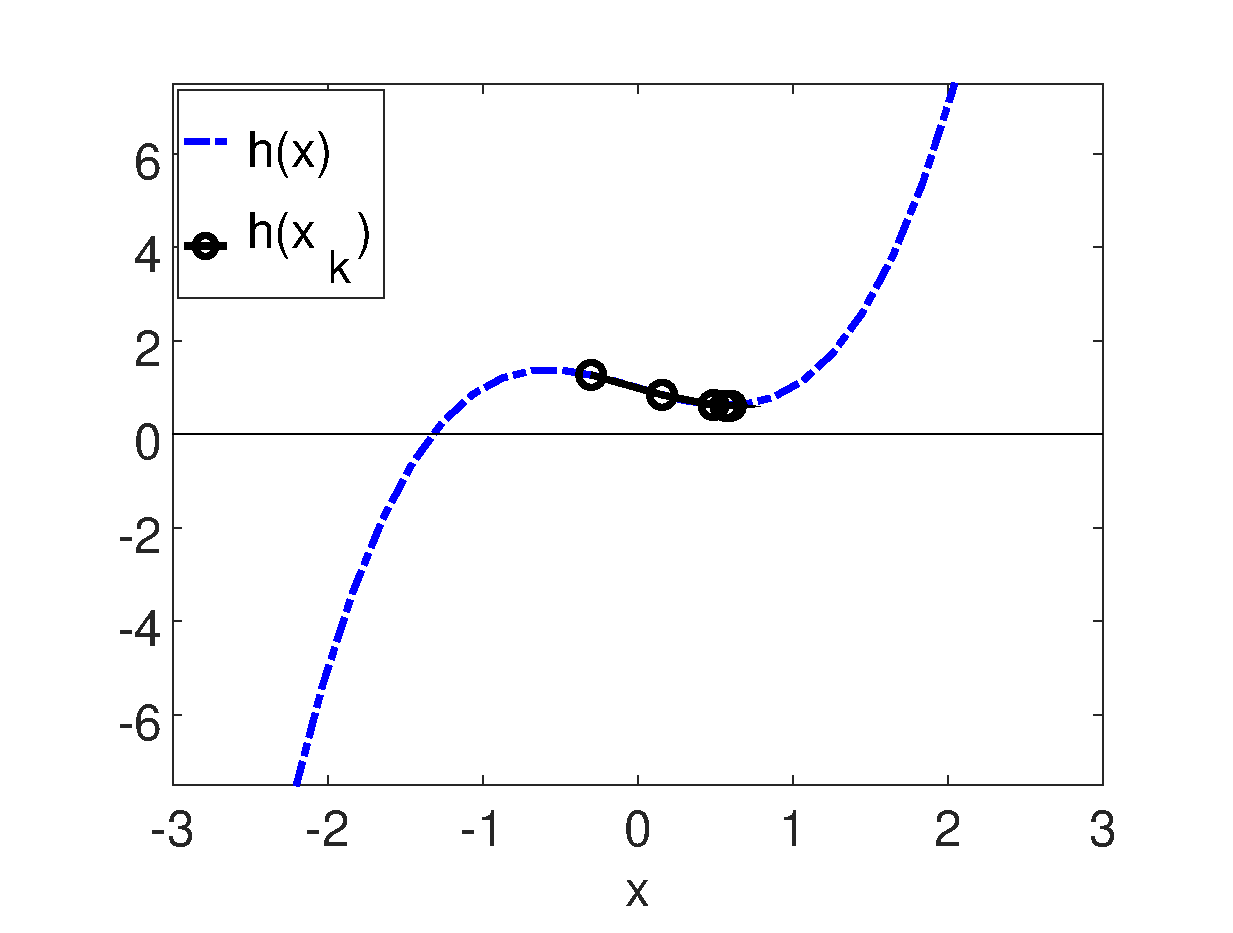
\includegraphics[width=\textwidth]{chapters/roots/mfiles/hx_a/minimizando_hx_a_1.eps}
        \caption{As iterações divergem ao redor de $x_m$, onde $h'(x_m)\approx 0$ e $h(x_m)\neq 0$.}
        \label{fig:rootsRcasesa}
    \end{subfigure}
    ~ %add desired spacing between images, e. g. ~, \quad, \qquad, \hfill etc. 
      %(or a blank line to force the subfigure onto a new line)
    \begin{subfigure}[b]{0.49\textwidth}
        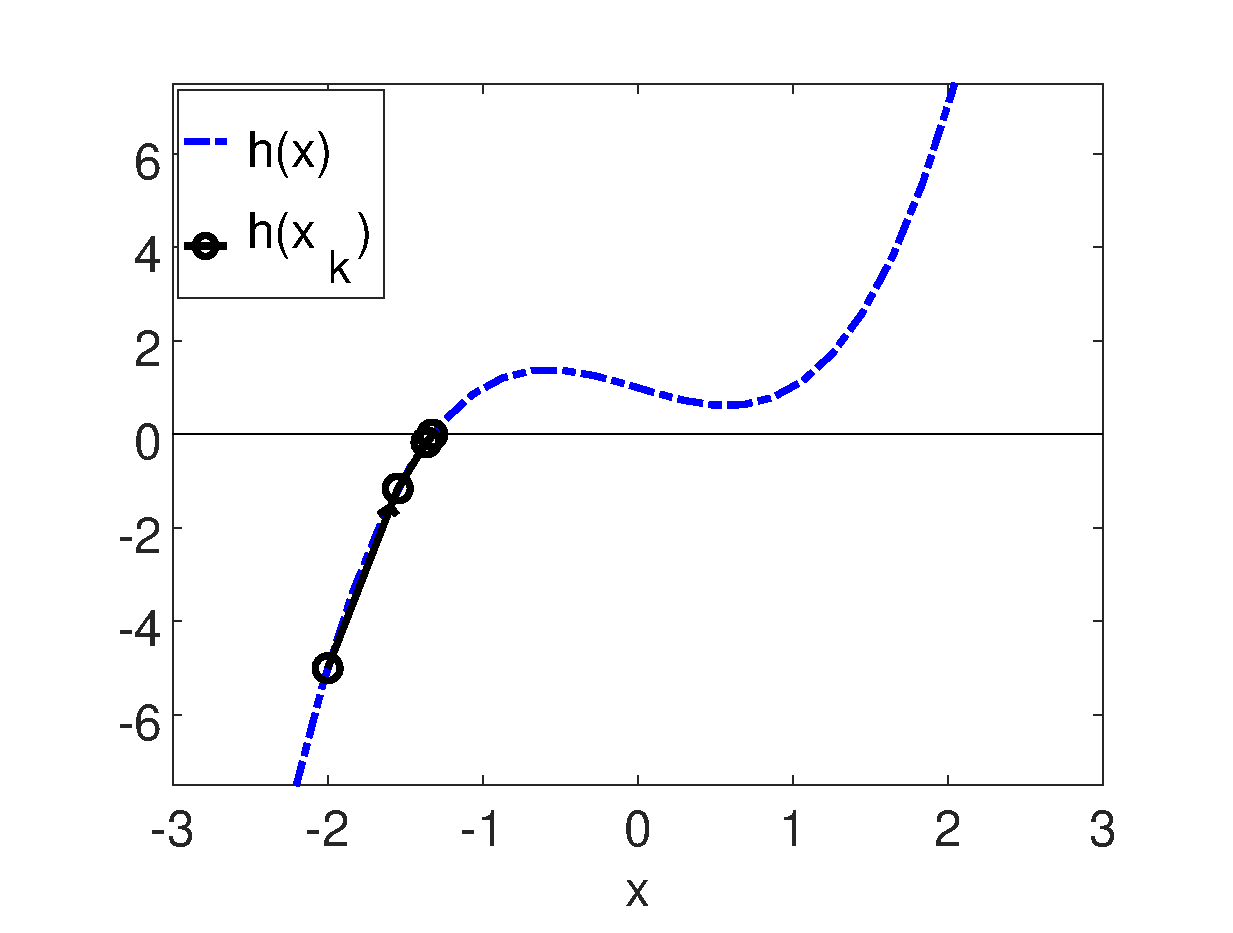
\includegraphics[width=\textwidth]{chapters/roots/mfiles/hx_a/minimizando_hx_a_2.eps}
        \caption{As iterações convergem em $\hat{x}$, onde $h(\hat{x})\approx 0$ e $h'(x_m)\neq 0$}
        \label{fig:rootsRcasesb}
    \end{subfigure}
    \caption{Comportamento da busca iterativa do Exemplo \ref{ex:rootshxreg1}}
    \label{fig:rootsRcases}
\end{figure}

\begin{table}[!h]
\centering
\begin{tabular}{|l|l|l|l|l|l|l|l|l|}
\hline
$k$      & 0 & 1 & 2 & 3 & 4 & 5 & 6 & 7\\ \hline
$x_k$    & -0.30000 & 0.15713 & 0.48972 & 0.60126 & 0.56670 & 0.58168 & 0.57551 & 0.57812 \\ \hline
$||h(x_k)||$ & 1.27300  & 0.84675 & 0.62773 & 0.61610 & 0.61530 & 0.61513 & 0.61511 & 0.61510 \\ \hline
\end{tabular}
\caption{Resposta iterativa do Exemplo \ref{ex:rootshxreg1}.}
\label{tab:rootsRcases1}
\end{table}

\begin{SolutionT}[Relativa ao Exemplo \ref{ex:rootshxreg1} (Converge errado):]\label{sol:rootshxreg2}
A Fig. \ref{fig:rootsRcasesb} nos mostra o processo de busca de uma raiz de $h(x)$. 
A busca inicia em $x_0=-2.0$,
 todos os valores $x_{k}$ podem ser vistos na Tabela \ref{tab:rootsRcases2}. 
Neste caso a busca iterativa indicada pela Eq. (\ref{eq:rootshxreg2}) converge 
em $\hat{x}\approx x_4 = -1.3248$ com $||h(x_4)||<\delta$ que corresponde a uma raiz de $h(x)$.
\end{SolutionT}

\begin{table}[!h]
\centering
\begin{tabular}{|l|l|l|l|l|l|}
\hline
$k$      & 0 & 1 & 2 & 3 & 4 \\ \hline
$x_k$    & -2.0000 & -1.5473 & -1.3626 & -1.3268 & -1.3248 \\ \hline
$||h(x_k)||$ & 5.0000e+00 & 1.1573e+00 & 1.6711e-01 & 9.0760e-03 & 2.5792e-04 \\ \hline
\end{tabular}
\caption{Resposta iterativa do Exemplo \ref{ex:rootshxreg1}.}
\label{tab:rootsRcases2}
\end{table}

